\subsection{Flexible Architekturen (Microservices)}

\subsubsection{Modelle}

\textbf{Monolith}

Nachteile
\begin{itemize}
    \item Einheitlicher langfristig einzusetzender Technologiestack
    \item \textcolor{blue}{erheblichen Koordinationsaufwand} Änderungen in der Architektur benötigen das Einverständnis bzw. Information aller, unter den Entwicklungsteams bei grosser fachlicher Breite für eine Applikation (z.B. ERP, CRM usw.), sowie der zentralen Stellen für das Deployment und Betrieb von Software
    \item Viele \textcolor{blue}{gegenseitige Abhängigkeiten} erschweren die Weiterentwicklung.
    \item \textcolor{blue}{Testing} betrifft alle Schichten und ganze Breite der Funktionalität. Daraus erfolgen Releasezyklen von mehreren Monaten
    \item Serverseitige \textcolor{blue}{Änderungen} und Erweiterungen für neue Technologien, wie z.B. Augmented Reality, IoT usw. stossen auf erhebliche Schwierigkeiten
    \item \textcolor{blue}{Deployment} ist komplex und kann nur in grösseren zeitlichen Abständen vorgenommen werden
    \item \textcolor{blue}{Migration} auf eine neue Technologie ist äussert
    aufwendig
\end{itemize}
\vspace{10pt}
\textbf{Self-Contained System (SCS) Microservices}

SCS nimmt eine vertikale Aufteilung der Applikation in fachliche Funktionen vor, wie z.B. Artikelservice, Kundenservice, Bestellservice usw. Enthalten alle notwendigen Schichten analog der Mehrschichtenarchitektur (Applikation wird in mehrere unabhängige Systeme aufgeteilt), jedes SCS ist eine unabhängige Web-Applikation mit eigenem GUI, Kommunikation zwischen SCS erfolgt per default asynchron, jedes SCS hat eigenständige Logik und Daten \\

Vorteile
\begin{itemize}
    \item lose Kopplung
    \item wenige Abhängigkeiten
    \item hohe Kohäsion
    \item wohldefinierte Aufgabe
\end{itemize}
\vspace{10pt}
\textbf{Microservice}

1 SCS kann aus 1-x Microservices bestehen, Bildet eine eigenständige fachlich klar fokussierte, eingegrenzten (Teil)funktion einer Applikation ab, Ihm steht ein eigener Ausführungscontainer/Laufzeitumgebung (Docker) zur Verfügung, Der Zugriff erfolgt über eine klar definierte synchrone und/oder asynchrone Schnittstelle \\

Vorteile
\begin{itemize}
    \item \textcolor{blue}{Klare fachliche Abgrenzung} mit sauberer Trennung der Zuständigkeiten je Service
    \item \textcolor{blue}{Lose Kopplung, möglichst Stateless} Ermöglicht einfaches Auswechseln der Komponenten
    \item \textcolor{blue}{Hohe Skalierung und Fehlertoleranz} Es können mehrere Scrum-
    Teams parallel an unterschiedlichen Microservices entwickeln
    \item \textcolor{blue}{Hohe technische Unabhängigkeit} Jedes Team hat innerhalb der für die Unternehmung strategisch festgelegten Plattformen die Freiheit, die optimale Technologie zu wählen
    \item \textcolor{blue}{Hohe Resilienz (Robustheit)} da Störung einer Komponente
    die anderen nicht beeinflussen
    \item \textcolor{blue}{Hohe Automatisierung} im CI/CD im DevOps-Kontext: \\ 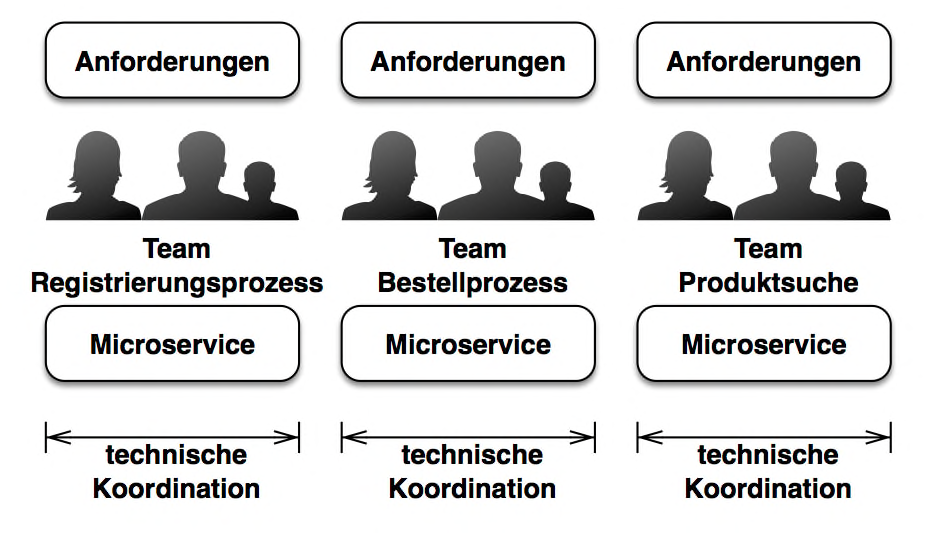
\includegraphics[width=\linewidth]{microservices-advantages.png}
\end{itemize}
\vspace{10pt}
Nachteile

\begin{itemize}
    \item Erhöhung der \textcolor{blue}{Gesamtkomplexität} durch die Zahl der Microservices
    \item Einsatz von \textcolor{blue}{unterschiedlichen Technologien} bedingt Erhalt des Knowhows $\rightarrow$ Verringert Flexibilität der Austauschbarkeit der Projektmitarbeiter
    \item \textcolor{blue}{Optimale Grösse} für Microservices muss gefunden werden (zu gross $\rightarrow$ Weiterentwicklung im gleichen Team kann nicht gewährleistet wer-
    den, zu klein $\rightarrow$ Komplexität der Interaktion und Abhängigkeiten steigen)
    \item \textcolor{blue}{Refactoring} das fachliche Teile von anderen Services herausschneidet, kann sehr aufwendig sein
    \item Lattenz beeinflusst die Performance negativ
\end{itemize}

\subsubsection{Domain Driven Design (DDD)}

Ist eine Vorgehensweise, um in komplexen Applikationen im strategischen Design die Fachdomänen mit klaren Kontextgrenzen herauszufinden und im taktischen Design im Detail zu spezifizieren.

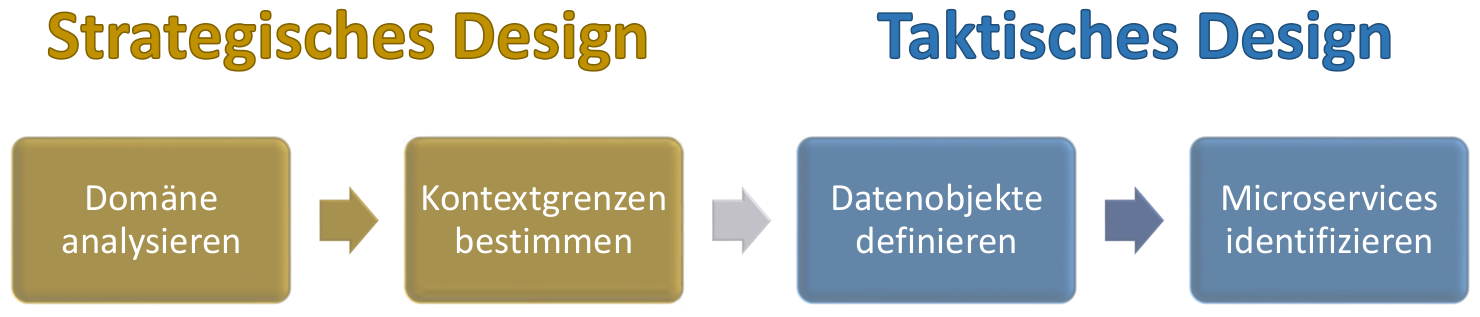
\includegraphics[width=\linewidth]{microservices-ddd.png} \\

\textbf{Strategisches Design}

\begin{itemize}
    \item Domäne analysieren
    \item Bounded Contexts festlegen (Fachlich klar abgegrenzter Kontext)
    \item Ubiquitous Language (Begriffe in einem Bounded Context) erarbeiten
    \item Context Map erstellen
\end{itemize}
\vspace{10pt}
\textbf{Taktisches Design}

\begin{itemize}
    \item (OO)-Entwurf in einem Bounded Context vornehmen
    \item Domain Events herausfinden
\end{itemize}
\vfill\null
\columnbreak
\subsubsection{Makroarchitektur}

\textbf{Persistenz}

Microservices haben eigene DB

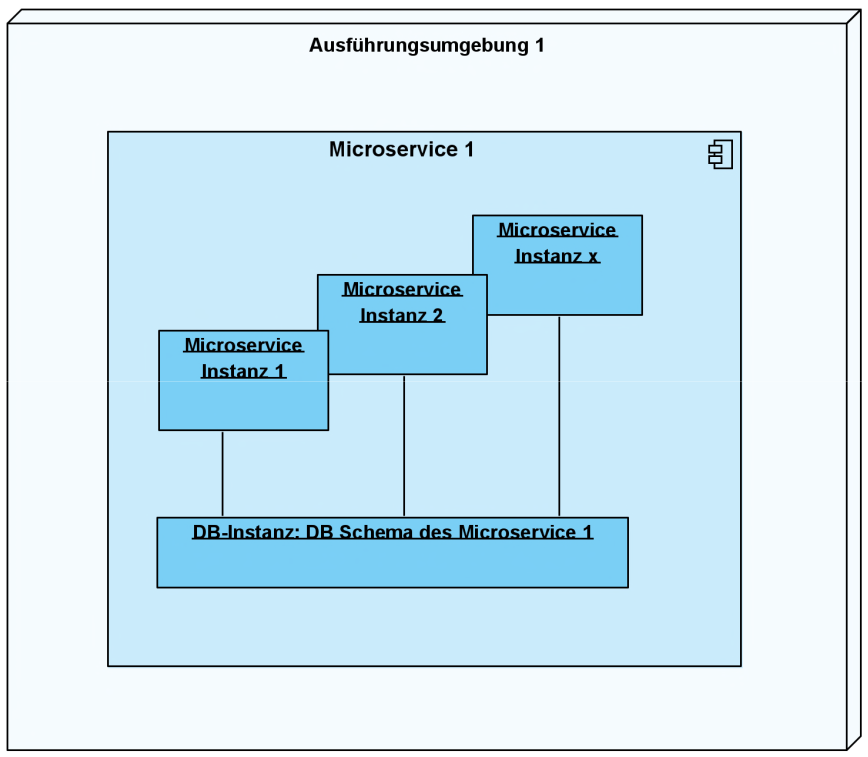
\includegraphics[width=0.8\linewidth]{microservices-persistence-1.png} \\

Zentraler DB-Service

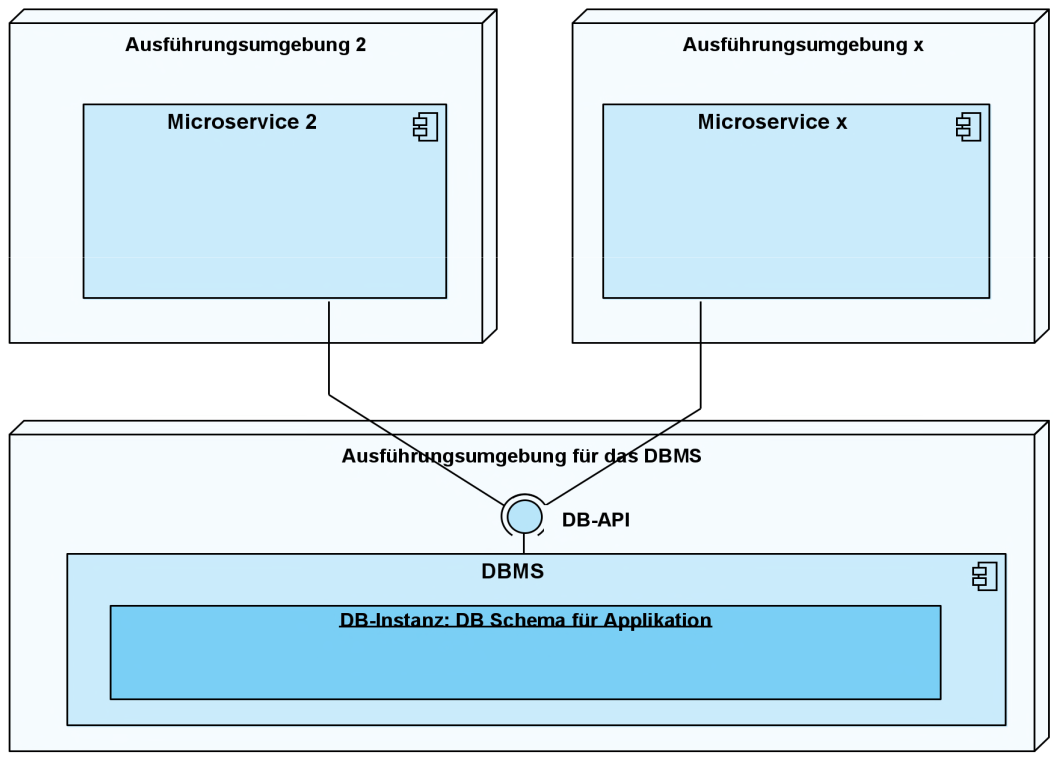
\includegraphics[width=0.8\linewidth]{microservices-persistence-2.png} \\

\textbf{Referenz-Makroarchitekturen}

\begin{itemize}
    \item \textcolor{blue}{API-Gateway} Bietet geeignete Web Service für Service Consumer an. Zugrunde liegende Middleware übernimmt Aufgaben wie Authentisierung, Atuorisierung, SSL/TLS-Endpoint, Web App Firewall (WAF), Logging, Service-
        Registry, Skalierung/Load-Balancing, Caching usw.
    \item \textcolor{blue}{Docker Host} Bietet für jeden Microservice Container an
    \item \textcolor{blue}{MOM} Messaging zwischen den Microservices erfolgt asynchron über einen Message Broker
    \item \textcolor{blue}{Shared Services} Microservices die allen anderen Microservices zur Verfügung stehen. Übernehmen meist Querschnittsfunktionen und können, eigene Persistenz enthalten
    \item \textcolor{blue}{Proxy Service} Übernimmt Kommunikation zu den applikationsexternen Service Provider und enthält meist eigenen Cache-Speicher
\end{itemize}
\vfill\null
\columnbreak
Full Server-Stack Microservices (Microservices als SCS)

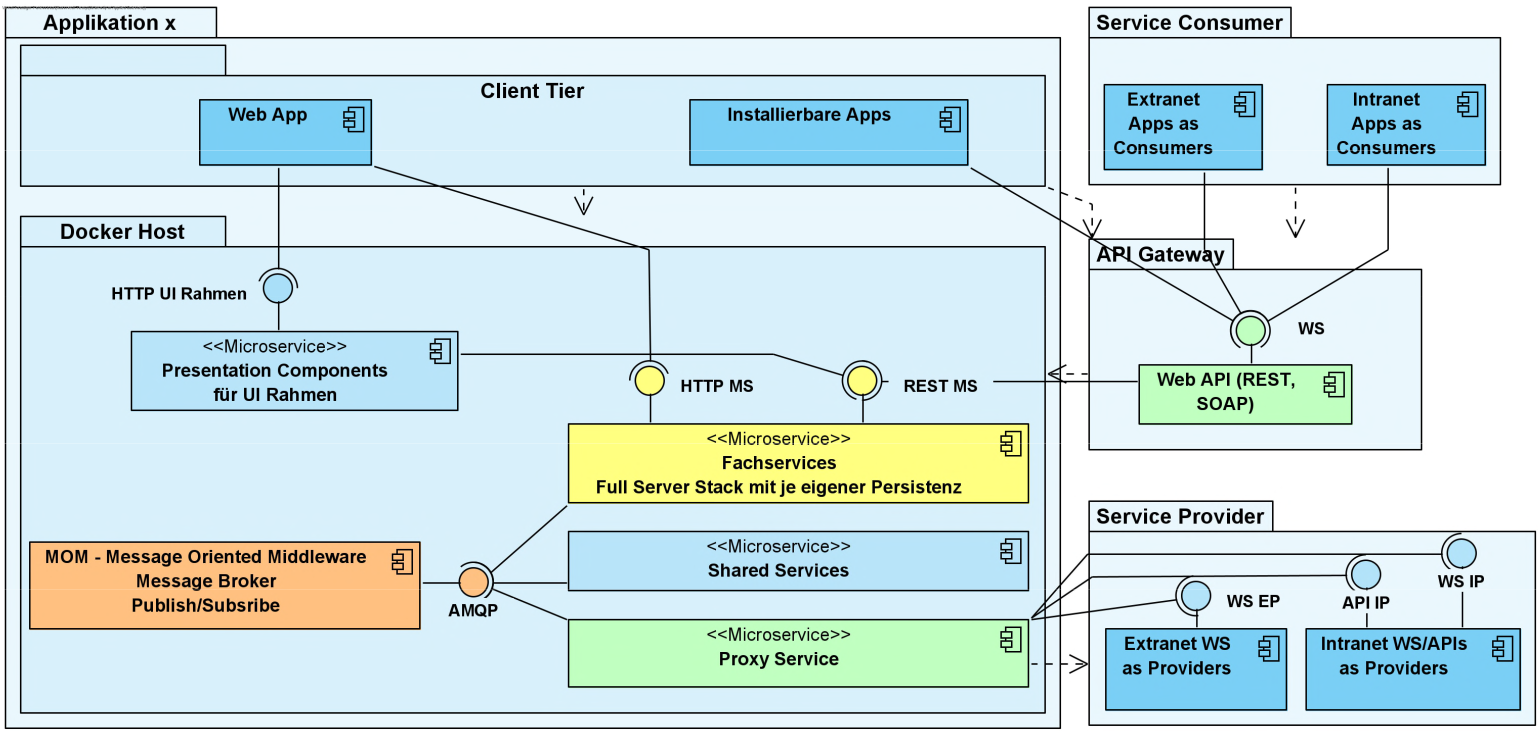
\includegraphics[width=\linewidth]{microservices-scs.png}

\begin{itemize}
    \item \textcolor{blue}{Client} UI Rahmen App und separate installierbare Client App (z.B. Mobile App)
    \item \textcolor{blue}{Persistenz} jeder Microservice hat eigene Persistenz
    \item \textcolor{blue}{Kommunikation} asynchrones Messaging über die MOM (Message Oriented Middleware), Zugriff auf Service Provider über einen zentralen proxy Microservice
\end{itemize}
\vspace{10pt}

\textbf{Beispiele}

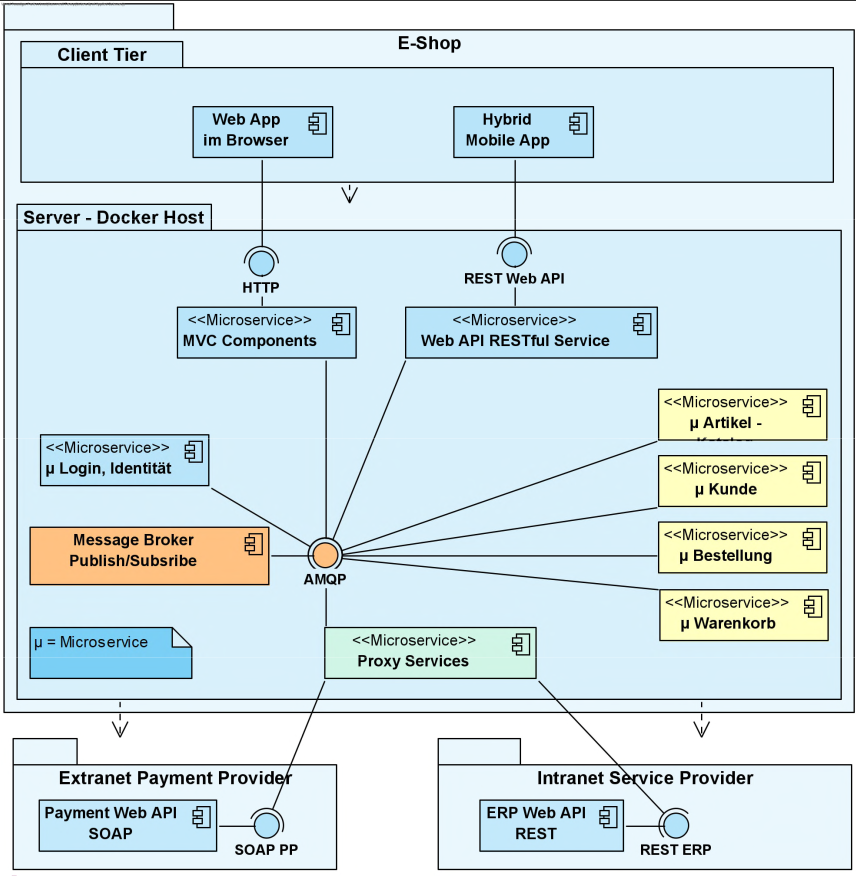
\includegraphics[width=\linewidth]{microservices-example.png}

\begin{itemize}
    \item \textcolor{blue}{API-Gateway} Da keine applikationsexterne Consumer vorgesehen sind, wird dieser weggelassen.
    \item \textcolor{blue}{Client Applikation} 2 Client Applikationen sind vorgesehen
    \begin{itemize}
        \item \textcolor{blue}{Web App} Kommuniziert mit MVC Components z.B. ASP.NET MVC
        \item \textcolor{blue}{Hybrid Mobile App} Kommuniziert mit Server über REST
    \end{itemize}
    \item \textcolor{blue}{Messaging} erfolgt asynchron über Message Broker mit dem AMQP-Protokoll
    \item \textcolor{blue}{Fachlogik} Ist auf 4 Microservices aufgeteilt. Jeder Microservice verfügt über eigene Persistenz.
    \item \textcolor{blue}{? Login, Identität} ist Querschnitts-Microservice, der Login-Daten persistent hält
    \item \textcolor{blue}{Proxy Services} Für die Kommunikation zu den beiden applikationsexternen Service Provider existieren je eine eigene Proxy-Komponente, welche in einem Microservice vereint sind
\end{itemize}
\vspace{10pt}
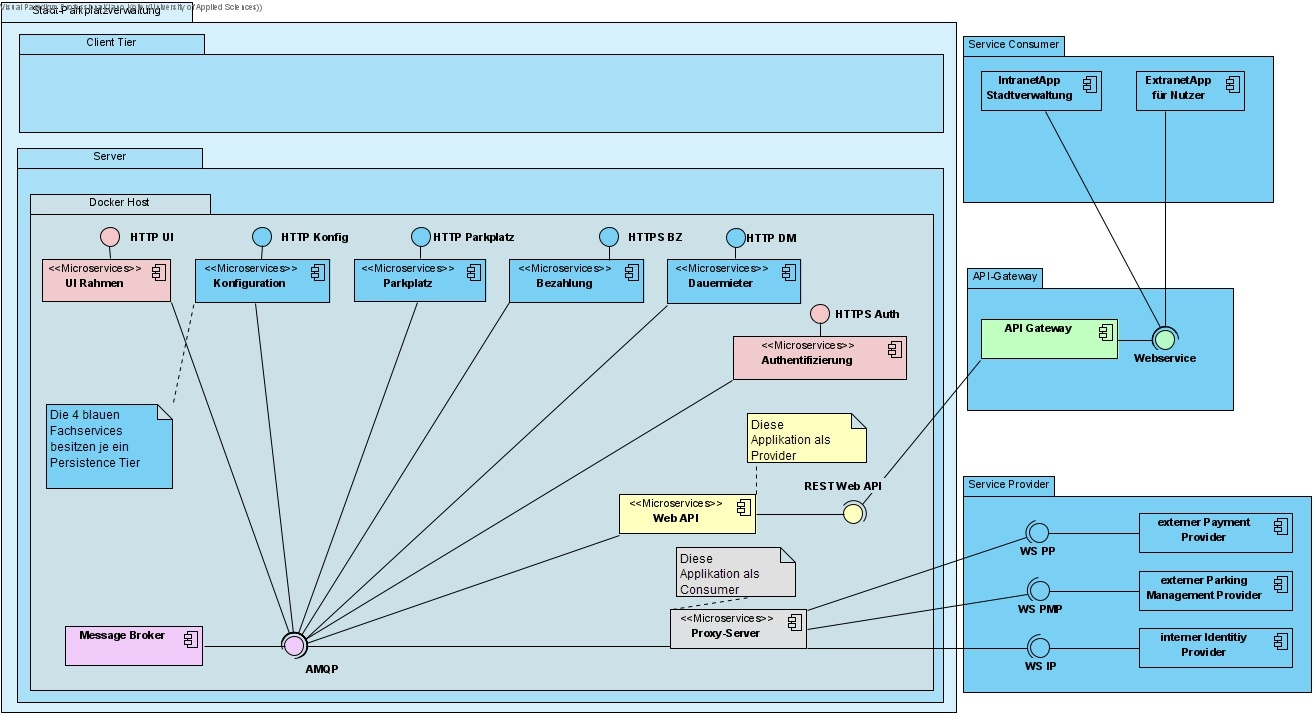
\includegraphics[width=\linewidth]{microservices-example-cars.png}

\subsubsection{Microarchitektur}

Jeder Mikroservices hat sein eigener Technologie-Stack, Dieser ist auf das zu beschränken, was benötigt wird

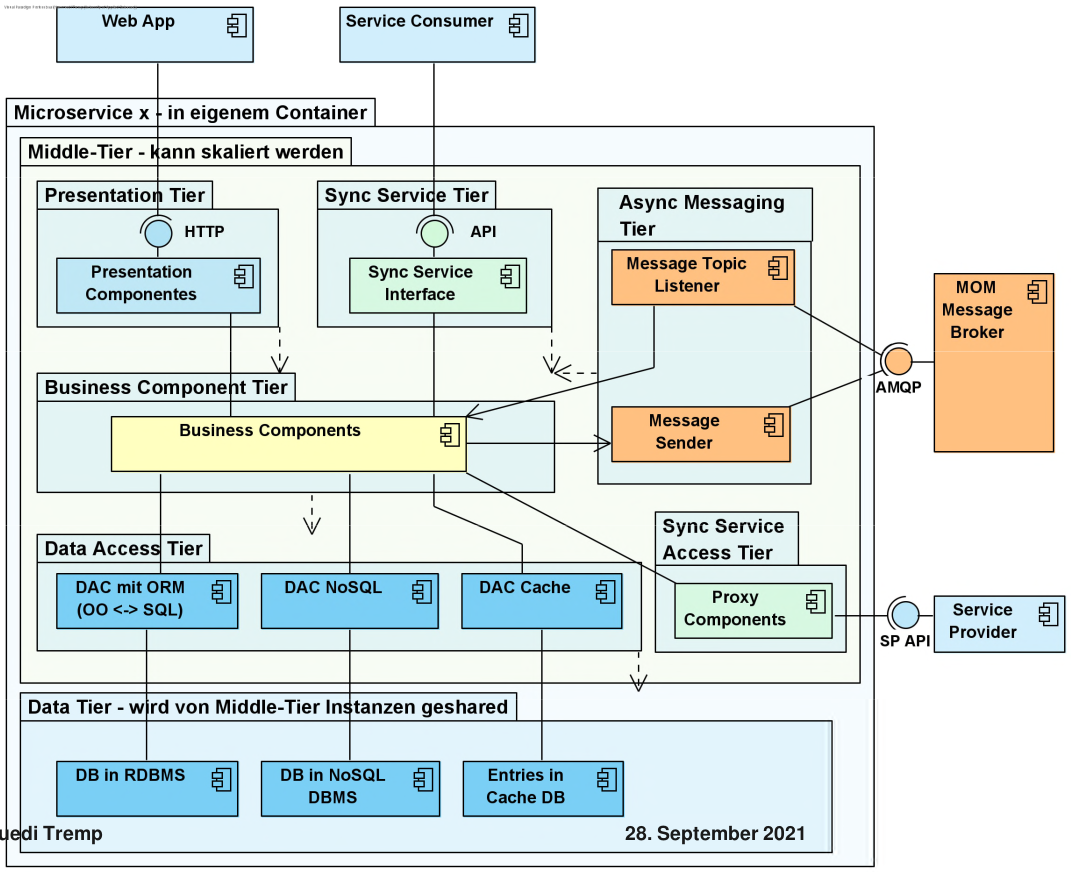
\includegraphics[width=\linewidth]{microservices-micro-architecture.png}

\subsubsection{Containerisierung}

mit Docker

\begin{itemize}
    \item Lifecycle-Management von Container: Planung, Konfiguration, Registrierung
    \item Provisionierung und Bereitstellung der Container
    \item Zuweisung der Ressourcen
    \item Skalierung der Container und Load-Balancer
    \item Sichern der Interaktion zwischen den Containern
    \item Monitoring
\end{itemize}

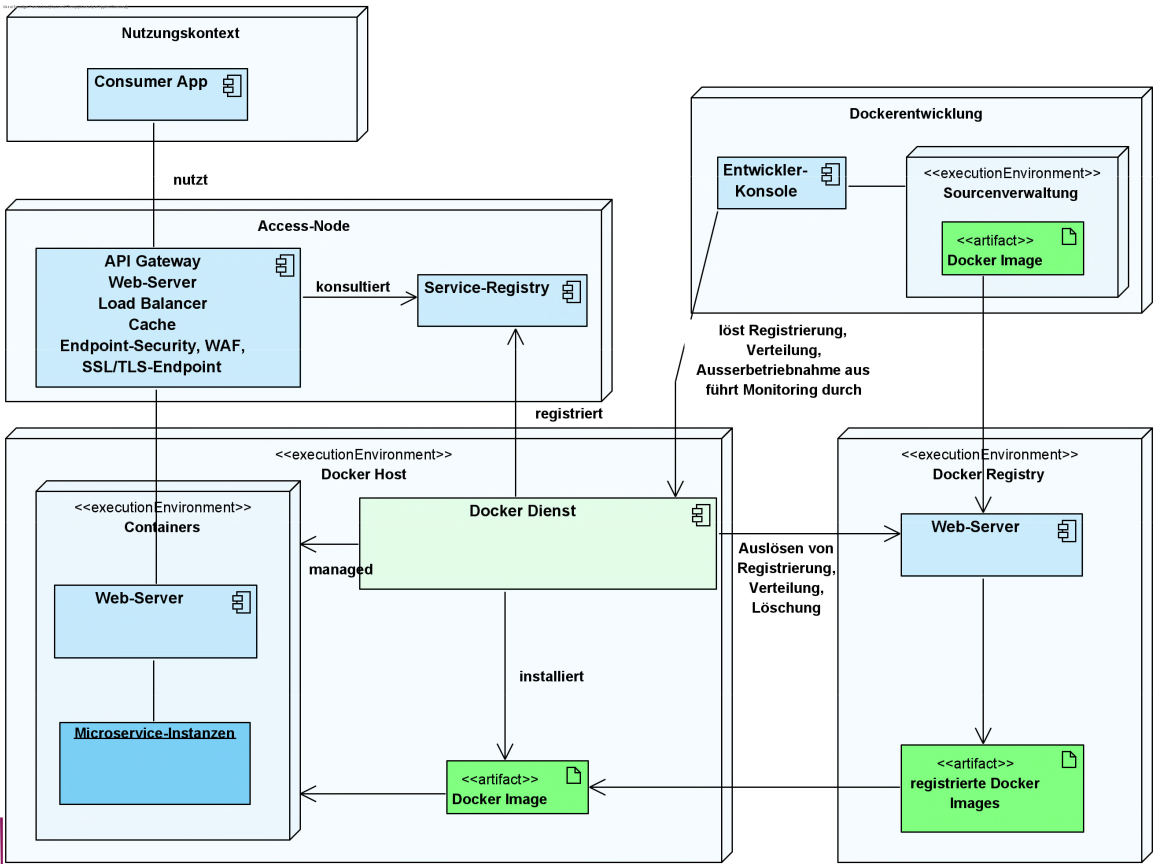
\includegraphics[width=\linewidth]{microservices-docker.png}

\columnbreak
\subsubsection{Prüfungsfragen}

\begin{itemize}
    \item Was spricht gegen ein applikationsweites kanonisches(gemeinsames) Datenmodell im Umfeld von Microservices? \\
    \textcolor{blue}{Erhaltung der Datenkonsistenz}
    \item Modellieren Sie eine Makro-Softwarearchitektur mit folgenden Elementen: Mobile-Client-App, API-Gateway, 3 Microservies, 1 Proxy-Microservice, 1 Extranet Web Service Provider \\
    \textcolor{blue}{Antwort}
    \item Inwiefern unterscheidet sich ein Container von einer VM? \\
    \textcolor{blue}{VM hat OS und Container nicht}
    \item Sie wollen hunderte von Ihren Microservices flexibel und sicher betreiben, CI/CD automatisieren, anhand des Traffics optimal skalieren und überwachen. Welche Art Software benötigen Sie dafür? Für welche konkrete Software entscheiden Sie sich? Geben Sie mindestens zwei Gute Gründe für Ihren Entscheid. \\
    \textcolor{blue}{Container-Orchestrierung $\rightarrow$ Kubernetes, weil es gut mit Docker harmonisiert}
\end{itemize}


